\section{Hardware Components and Construction}

Comparative measurements were carried out to choose the elements composing the CND. The tests were geared towards optimizing the time resolution, which is the key parameter to ensure $n/\gamma$ separation, and containing all associated costs. 
Different prototypes were constructed and employed for measurements of time resolution and light-yield during cosmic ray testing to optimize the final design choices for scintillator type, PMT, wrapping material, PMT magnetic shielding configuration, shape of the U-turn light guide, and glue for the optical coupling. The outcomes of these tests are discussed in detail in \cite{Niccolai:2018qzm}.
The chosen components are:
\begin{itemize}
\item{144 EJ200 scintillator bars, by Eljen Technology;}
\item{144 Hamamatsu R10533 2-in PMTs;}
\item{72 semi-circular-shaped U-turn light guides of Polymethyl Methacrylate (PMMA);
\item{aluminum foil as reflector material wrapping the scintillator bars;}
}
\item{a 1-mm-thick mu-metal cylinder plus a 5-mm-thick mild steel cylinder to shield each PMT from the stray magnetic field of the CLAS12 solenoid;}
\item{coupling with optical grease between PMT and light guide;}
\item{M-Bond200 glue for the junctions between scintillators and light guides.}
\end{itemize}

The 24 blocks composing the Central Neutron Detector were assembled in the mechanical shop of IPN Orsay \cite{Niccolai:2018qzm} and then shipped to Jefferson Lab (JLab), along with the components of the support structure. The support structure consists of six separate aluminum arches that are fastened together to form a ring, which is in turn attached to the solenoid by means of stainless-steel brackets. 
The support structure was installed first onto the CLAS12 solenoid, and then the 24 blocks of the CND were inserted, one by one, and secured onto the structure. The PMTs, within their shieldings, were then connected to the end of the light guides, to which they were coupled with optical grease. Figure~\ref{photo_cnd_installed} shows the detector after its installation. 
\begin{figure}[htb]
\begin{center}
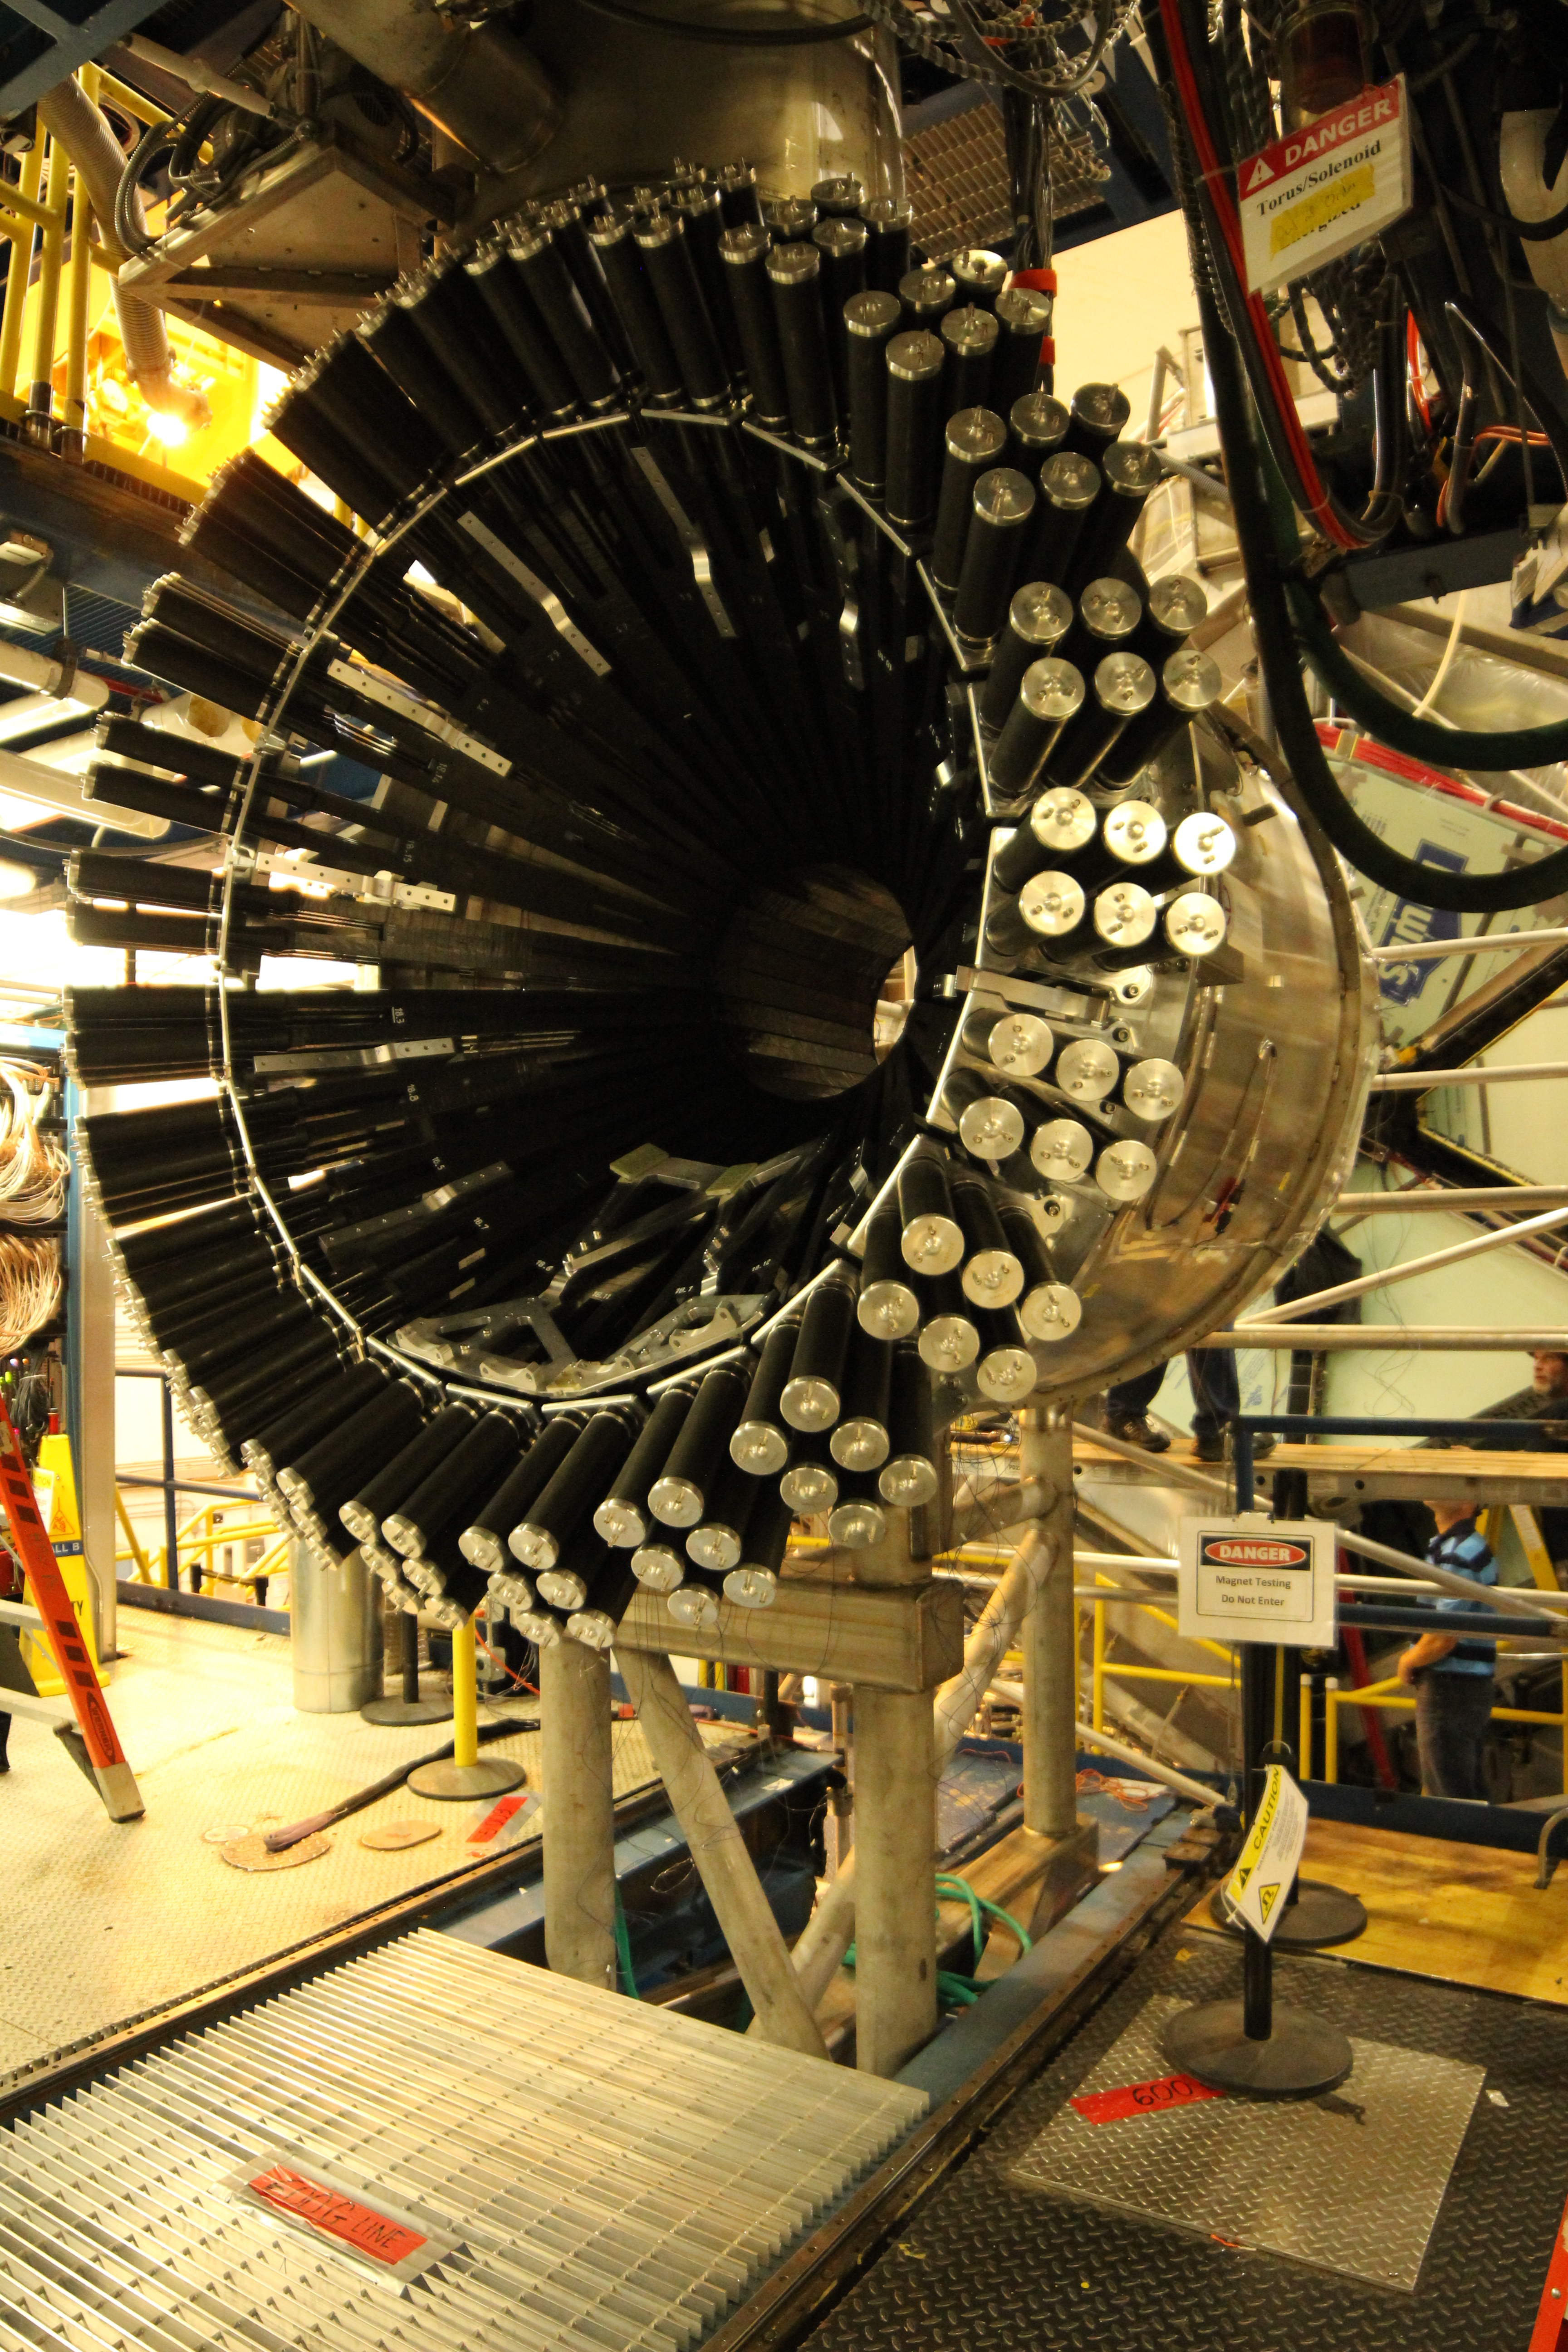
\includegraphics[width=0.35\textwidth]{Figure/IMG_4878.JPG} 
\end{center}
\caption{The Central Neutron Detector as installed in the CLAS12 solenoid.}
\label{photo_cnd_installed}
\end{figure}
